\documentclass[12pt,letterpaper]{article}
\usepackage{graphicx,textcomp}
\usepackage{natbib}
\usepackage{setspace}
\usepackage{fullpage}
\usepackage{color}
\usepackage[reqno]{amsmath}
\usepackage{amsthm}
\usepackage{fancyvrb}
\usepackage{amssymb,enumerate}
\usepackage[all]{xy}
\usepackage{endnotes}
\usepackage{lscape}
\newtheorem{com}{Comment}
\usepackage{float}
\usepackage{hyperref}
\newtheorem{lem} {Lemma}
\newtheorem{prop}{Proposition}
\newtheorem{thm}{Theorem}
\newtheorem{defn}{Definition}
\newtheorem{cor}{Corollary}
\newtheorem{obs}{Observation}
\usepackage[compact]{titlesec}
\usepackage{dcolumn}
\usepackage{tikz}
\usetikzlibrary{arrows}
\usepackage{multirow}
\usepackage{xcolor}
\newcolumntype{.}{D{.}{.}{-1}}
\newcolumntype{d}[1]{D{.}{.}{#1}}
\definecolor{light-gray}{gray}{0.65}
\usepackage{url}
\usepackage{listings}
\usepackage{color}
\usepackage{enumitem}
\usepackage{booktabs}

\definecolor{codegreen}{rgb}{0,0.6,0}
\definecolor{codegray}{rgb}{0.5,0.5,0.5}
\definecolor{codepurple}{rgb}{0.58,0,0.82}
\definecolor{backcolour}{rgb}{0.95,0.95,0.92}

\lstdefinestyle{mystyle}{
	backgroundcolor=\color{backcolour},   
	commentstyle=\color{codegreen},
	keywordstyle=\color{magenta},
	numberstyle=\tiny\color{codegray},
	stringstyle=\color{codepurple},
	basicstyle=\footnotesize,
	breakatwhitespace=false,         
	breaklines=true,                 
	captionpos=b,                    
	keepspaces=true,                 
	numbers=left,                    
	numbersep=5pt,                  
	showspaces=false,                
	showstringspaces=false,
	showtabs=false,                  
	tabsize=2
}
\lstset{style=mystyle}
\newcommand{\Sref}[1]{Section~\ref{#1}}
\newtheorem{hyp}{Hypothesis}

\title{Problem Set 3}
\date {Name: Darragh McGee (18319331)\\}
\author{Applied Stats/Quant Methods 1}

\vspace{2.5cm}

\begin{document}
	\maketitle
	\vspace{.5cm}
\section*{Question 1}
\vspace{.25cm}
\noindent We are interested in knowing how the difference in campaign spending between incumbent and challenger affects the incumbent's vote share. 
\noindent\begin{enumerate}[left=0pt]
\item Run a regression where the outcome variable is \texttt{voteshare} and the explanatory variable is 
\texttt{difflog}.
\end{enumerate}

\vspace{0.5cm}
\noindent\textbf{Linear Regression Assumptions}
\begin{itemize}[left=0pt]
	\item 
	\textbf{Linear Relationship:} There is a linear relationship between the outcome and explanatory variables.
	\item
	\textbf{Independence of Errors:} The errors (residuals) are independent of each other.
	\item 
	\textbf{Normality of errors:} For any given value of the explanatory variable, the errors (residuals) are assumed to follow a normal distribution.
	\item
	\textbf{Constant variance (Homoscedasticity)}: The variance of the errors is constant across all values of the explanatory variable. 
	\item
	\textbf{No Perfect Multi-Collinearity:} The explanatory variables should not be perfectly correlated with each other. 
\end{itemize}
\vspace{0.5cm}	

\noindent Read in Data:
\lstinputlisting[language=R, firstline=5, lastline=5]{PS3_answers_DMcG.R}

\newpage
\noindent Regression Model (1) for \texttt{voteshare} and \texttt{difflog}: 
\noindent\lstinputlisting[language=R, firstline=22, lastline=23]{PS3_answers_DMcG.R}

\begin{table}[h!]
	\centering
	\caption{Summary of Model 1 Regression Results}
	\vspace{0.25cm}
	\begin{tabular}{lccc}
		\toprule
		\textbf{Variable} & \textbf{Estimate} & \textbf{Std. Error} & \textbf{Significance} \\ 
		\midrule
		Intercept              & 0.579031 & 0.002251 & *** \\ 
		presvote               & 0.041666 & 0.000968 & *** \\ 
		\midrule
		\textbf{Model Summary} & & & \\
		Residual Std. Error    & 0.07867  & & \\ 
		Multiple R-squared     & 0.3673   & & \\ 
		Adjusted R-squared     & 0.3671   & & \\ 
		Number of Observations & 3192     & & \\ 
		\bottomrule
	\end{tabular}
\end{table}

\vspace{0.1cm}
\noindent\textbf{Significance Codes:} \\
*** $p < 0.001$, ** $p < 0.01$, * $p < 0.05$
	
\vspace{0.5cm} \begin{itemize}[left=0pt, label=\textbullet]
\item The intercept of 0.579031 indicates that when the logarithmic difference in campaign spending between the incumbent and challenger (\texttt{difflog}) is zero, the incumbent's predicted vote share (\texttt{voteshare}) is 57.9 percent.
\item There is a positive, statistically significant relationship between \texttt{difflog} and \texttt{voteshare}, with a p-value of less than 0.001 (indicated by three stars in the regression table).
\item Specifically, a one-unit increase in \texttt{difflog} is associated with an average increase of 0.04 (or 4 percentage points) in \texttt{voteshare}. 
\end{itemize}

\newpage
	\begin{enumerate}[left=0pt]
	\setcounter{enumi}{1}
		\item Make a scatterplot of the two variables and add the regression line.
	\end{enumerate}

\noindent Code to Plot the Relationship:
\lstinputlisting[language=R, firstline=38, lastline=43]{PS3_answers_DMcG.R}
\begin{figure}[H]
	\centering
	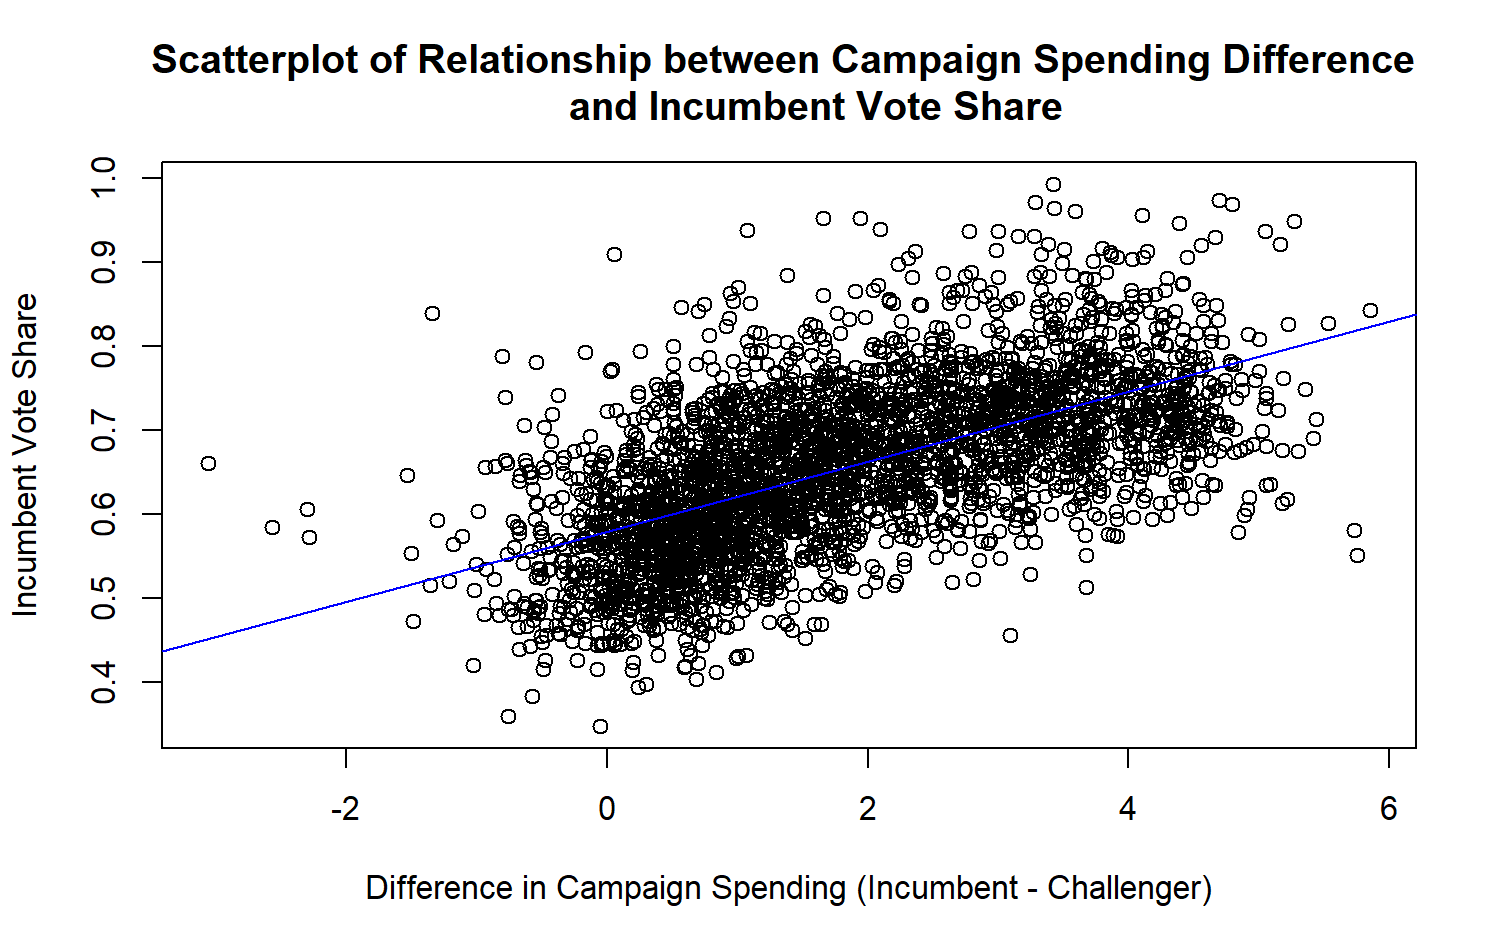
\includegraphics[width=1\textwidth]{Figure_1_1.png}
\end{figure}
	
\newpage	
\begin{enumerate}[left=0pt]
	\setcounter{enumi}{2}
		\item Save the residuals of the model in a separate object.
	\end{enumerate}
	
\noindent Save Residuals as a Separate Object:
\lstinputlisting[language=R, firstline=48, lastline=48]{PS3_answers_DMcG.R}
	\begin{enumerate}[left=0pt]
	\setcounter{enumi}{3}
	
	\item Write the prediction equation.
	\end{enumerate}

Below is the Typical Linear Regression Prediction Equation Structure: 
\begin{equation}
	\hat{y} = \hat{\beta}_0 + \hat{\beta}_1 x_1 + \hat{\beta}_2 x_2 + \dots + \hat{\beta}_p x_p
\end{equation}

where:
\begin{itemize}
	\item $\hat{y}$ is the predicted value of the outcome variable,
	\item $\hat{\beta}_0$ is the estimated intercept,
	\item $\hat{\beta}_1, \hat{\beta}_2, \dots, \hat{\beta}_p$ are the estimated coefficients for each explanatory variable,
	\item $x_1, x_2, \dots, x_p$ are the explanatory variables.
\end{itemize}

\vspace{0.25cm}
\noindent The first model is a bivariate model meaning there is a single outcome and explanatory variable.  \texttt{voteshare} is the outcome variable and  \texttt{difflog} is the explanatory variable. 

\begin{equation}
	{\text{voteshare}} = \hat{\beta}_0 + \hat{\beta}_1 \cdot \text{difflog}
\end{equation}

\vspace{0.5cm} \noindent Inputting the Values from Model 1 Regression Output:
\begin{equation}
	{\text{voteshare}} = 0.5709 + 0.4167 \cdot \text{difflog}
\end{equation}
	
\newpage

\section*{Question 2}
\noindent We are interested in knowing how the difference between incumbent and challenger's spending and the vote share of the presidential candidate of the incumbent's party are related.	\vspace{.25cm}
\noindent\begin{enumerate}[left=0pt]
\item Run a regression where the outcome variable is \texttt{presvote} and the explanatory variable is \texttt{difflog}.
\end{enumerate}
\vspace{0.5cm}	
\noindent Regression Model (2) for \texttt{presvote} and \texttt{difflog}:
\noindent\lstinputlisting[language=R, firstline=56, lastline=57]{PS3_answers_DMcG.R}

\begin{table}[h!]
	\centering
	\caption{Summary of Model 2 Regression Results}
	\vspace{0.25cm}
	\begin{tabular}{lccc}
		\toprule
		\textbf{Variable} & \textbf{Estimate} & \textbf{Std. Error} & \textbf{Significance} \\ 
		\midrule
		Intercept              & 0.507583 & 0.003161 & *** \\ 
		difflog                & 0.023837 & 0.001359 & *** \\ 
		\midrule
		\textbf{Model Summary} & & & \\
		Residual Std. Error    & 0.07867  & (df = 3191) & \\ 
		Multiple R-squared     & 0.3673   & & \\ 
		Adjusted R-squared     & 0.3671   & & \\ 
		Number of Observations & 3192     & & \\ 
		\bottomrule
	\end{tabular}
\end{table}

\vspace{0.1cm}
\noindent\textbf{Significance Codes:} \\
*** $p < 0.001$, ** $p < 0.01$, * $p < 0.05$

\vspace{0.5cm} \begin{itemize}[left=0pt, label=\textbullet]
	\item The intercept of 0.5075 indicates that when the logarithmic difference in campaign spending between the incumbent and challenger (\texttt{difflog}) is zero, the predicted vote share of the presidential candidate of the incumbent (\texttt{presvote}) is 50.75 percent.
	
	\item There is a positive, statistically significant relationship between \texttt{difflog} and \texttt{presvote}, with a p-value of less than 0.001 (indicated by three stars in the regression table).
	
	\item Specifically, a one-unit increase in \texttt{difflog} is associated with an average increase of 0.0238 (or 2.38 percentage points) in the vote share of the presidential candidate of the incumbent.
\end{itemize}
\newpage
\vspace{0.5cm}\noindent\begin{enumerate}[left=0pt]	
\setcounter{enumi}{1}	
		\item Make a scatterplot of the two variables and add the regression line.
\end{enumerate}

\noindent Code to Plot the Relationship:
\lstinputlisting[language=R, firstline=74, lastline=79]{PS3_answers_DMcG.R}
\begin{figure}[H]
	\centering
	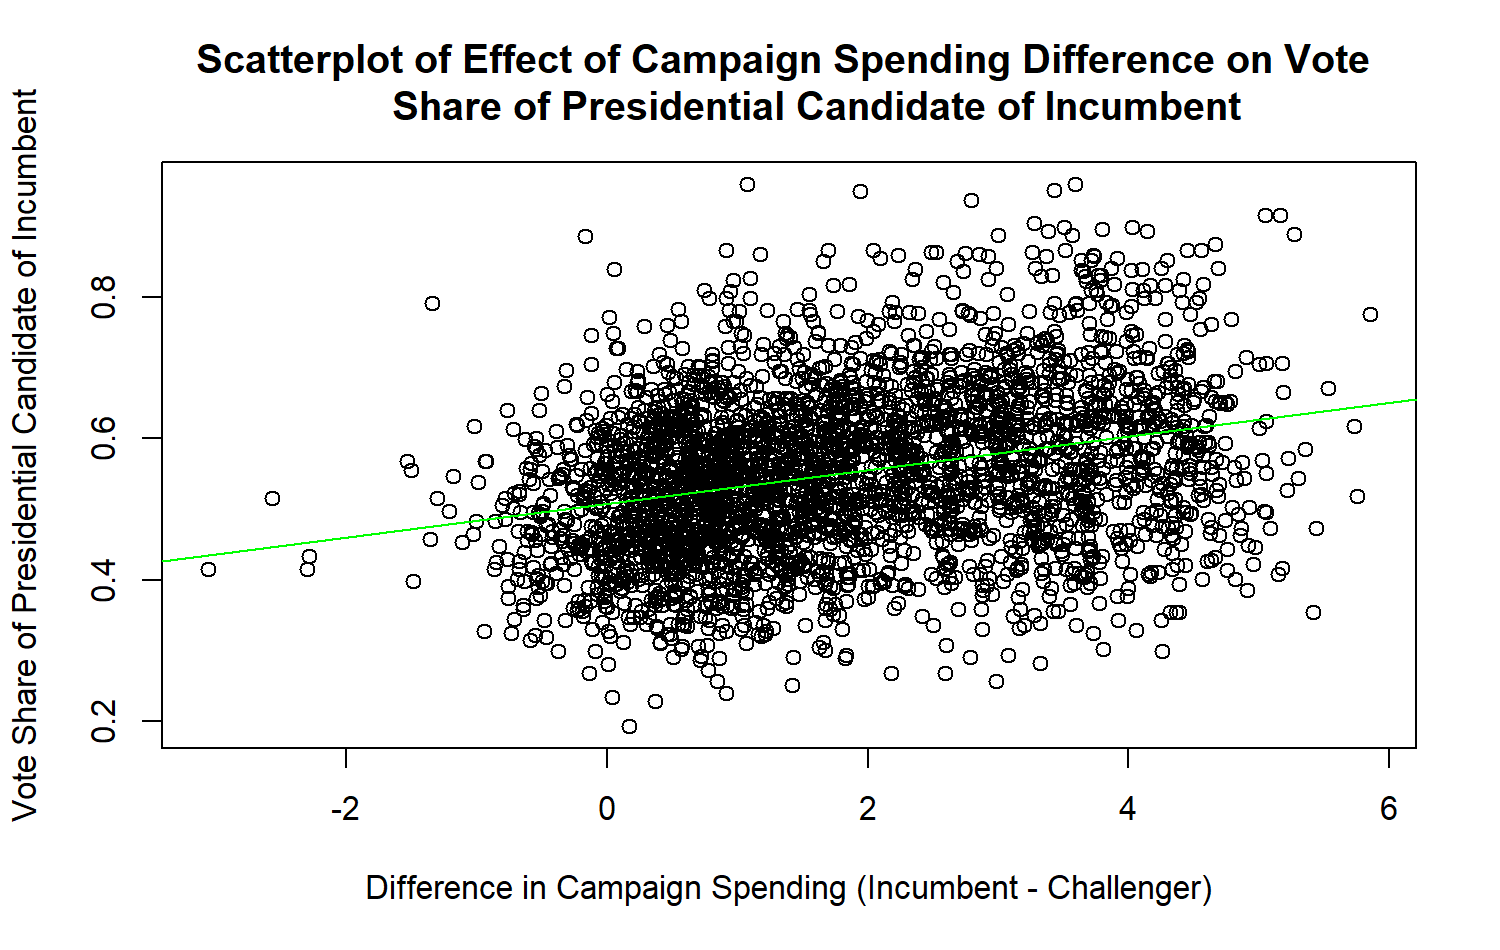
\includegraphics[width=1\textwidth]{Figure_2_1.png}
\end{figure}

\noindent\begin{enumerate}[left=0pt]		
\setcounter{enumi}{2} 
		\item Save the residuals of the model in a separate object.
	\end{enumerate}
	
	\noindent Save Residuals as a Separate Object:
	\lstinputlisting[language=R, firstline=83, lastline=83]{PS3_answers_DMcG.R}

\newpage		
\noindent\begin{enumerate}[left=0pt]
\setcounter{enumi}{3}		
		\item Write the prediction equation.
	\end{enumerate}
	
\noindent The second model is a bivariate model, meaning there is a single outcome and explanatory variable.  \texttt{presvote} is the outcome variable, and  \texttt{difflog} is the explanatory variable.

\begin{equation}
	\text{presvote} = \hat{\beta}_0 + \hat{\beta}_1 \cdot \text{difflog}
\end{equation}

\vspace{0.5cm} \noindent Inputting the values from the Model 2 Regression Output:
\begin{equation}
	\text{presvote} = 0.5076 + 0.0238 \cdot \text{difflog}
\end{equation}
	
	\newpage	
\section*{Question 3}

\noindent We are interested in knowing how the vote share of the presidential candidate of the incumbent's party is associated with the incumbent's electoral success.
\vspace{.25cm}
\noindent\begin{enumerate}[left=0pt]
		\item Run a regression where the outcome variable is \texttt{voteshare} and the explanatory variable is \texttt{presvote}.		

\vspace{0.5cm}	
\noindent Regression Model (3) for \texttt{voteshare} and \texttt{presvote}:
\noindent\lstinputlisting[language=R, firstline=91, lastline=93]{PS3_answers_DMcG.R}

\begin{table}[h!]
	\centering
	\caption{Summary of Model 3 Regression Results}
	\vspace{0.25cm}
	\begin{tabular}{lccc}
		\toprule
		\textbf{Variable} & \textbf{Estimate} & \textbf{Std. Error} & \textbf{Significance} \\ 
		\midrule
		Intercept              & 0.441330 & 0.007599 & *** \\ 
		presvote               & 0.388018 & 0.013493 & *** \\ 
		\midrule
		\textbf{Model Summary} & & & \\
		Residual Std. Error    & 0.08815  & (df = 3191) & \\ 
		Multiple R-squared     & 0.2058   & & \\ 
		Adjusted R-squared     & 0.2056   & & \\ 
		Number of Observations & 3192     & & \\ 
		\bottomrule
	\end{tabular}
\end{table}

\vspace{0.1cm}
\noindent\textbf{Significance Codes:} \\
*** $p < 0.001$, ** $p < 0.01$, * $p < 0.05$

\vspace{0.5cm} \begin{itemize}[left=0pt, label=\textbullet]
	\item The intercept of 0.4413 indicates that when the vote share of the incumbent’s presidential candidate (\texttt{presvote}) is zero, the predicted vote share of the incumbent (\texttt{voteshare}) is 44.13 percent.
	
	\item There is a positive, statistically significant relationship between \texttt{presvote} and \texttt{voteshare}, with a p-value of less than 0.001 (indicated by three stars in the regression table).
	
	\item Specifically, a one-unit increase in \texttt{presvote} is associated with an average increase of 0.388 (or 38.8 percentage points) in \texttt{voteshare}.
\end{itemize}

\end{enumerate}
\newpage
\noindent\begin{enumerate}[left=0pt]
\setcounter{enumi}{1}	
		\item Make a scatterplot of the two variables and add the regression line. 
\end{enumerate}		

\noindent Code to Plot the Relationship:
\lstinputlisting[language=R, firstline=106, lastline=107]{PS3_answers_DMcG.R}
\begin{figure}[H]
	\centering
	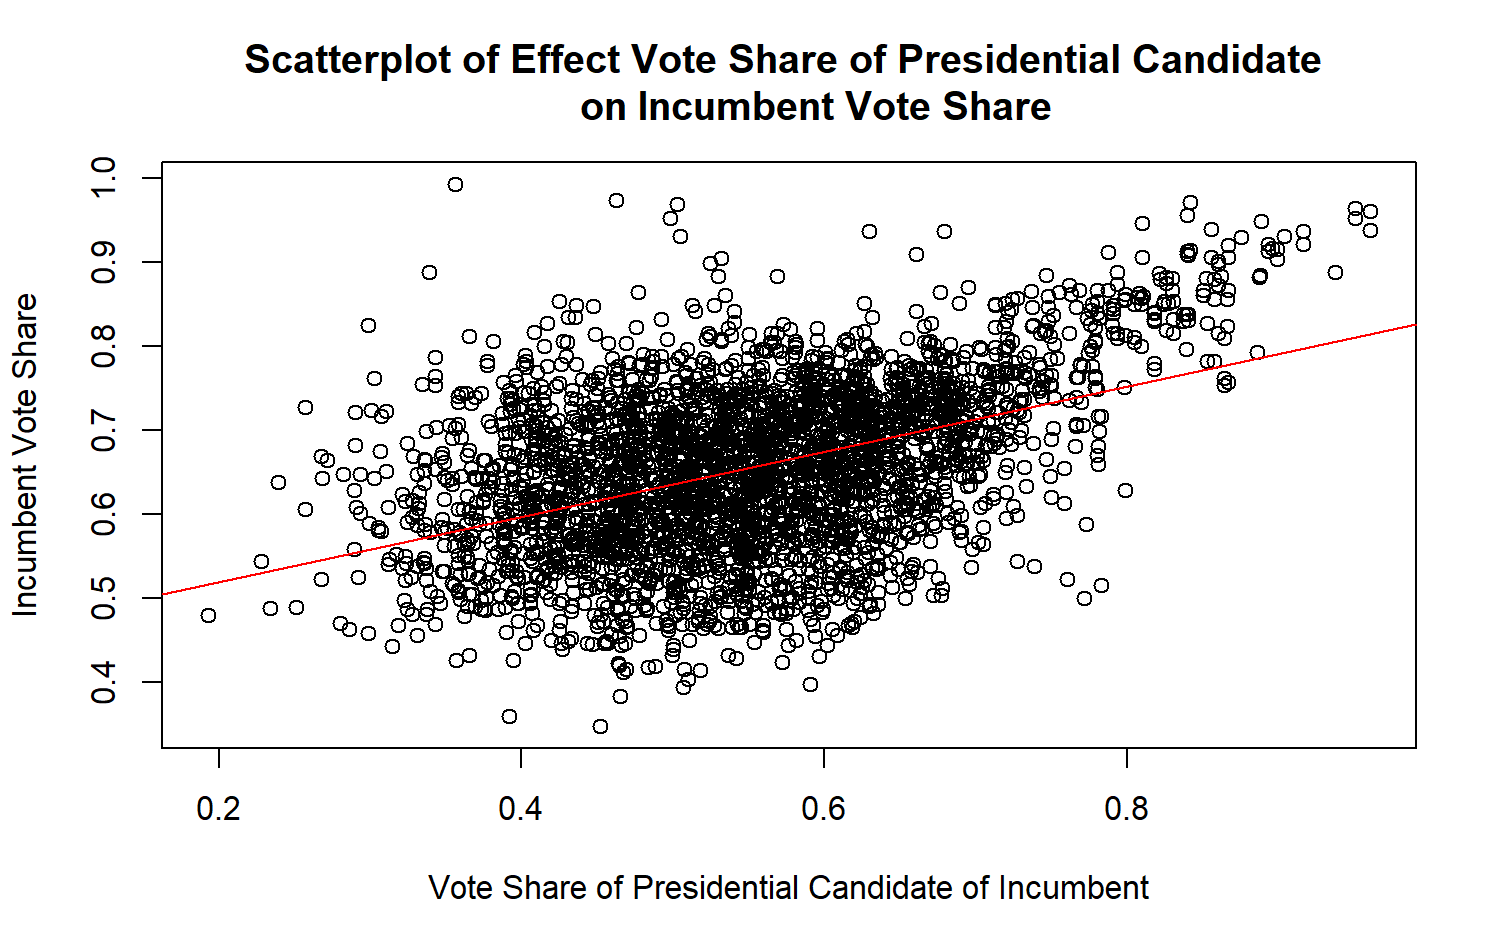
\includegraphics[width=1\textwidth]{Figure_3_1.png}
\end{figure}

\noindent\begin{enumerate}[left=0pt]		
\setcounter{enumi}{2}	
		\item Write the prediction equation.
	\end{enumerate}
	
\vspace{0.25cm}
\noindent The third model is a bivariate model, meaning there is a single outcome and explanatory variable.  \texttt{voteshare} is the outcome variable, and  \texttt{presvote} is the explanatory variable.

\begin{equation}
	\text{voteshare} = \hat{\beta}_0 + \hat{\beta}_1 \cdot \text{presvote}
\end{equation}

\vspace{0.5cm} \noindent Inputting the values from the Model 3 Regression Output:
\begin{equation}
	\text{voteshare} = 0.4413 + 0.3880 \cdot \text{presvote}
\end{equation}

\newpage	
\section*{Question 4}
\noindent The residuals from part (a) tell us how much of the variation in \texttt{voteshare} is $not$ explained by the difference in spending between incumbent and challenger. The residuals in part (b) tell us how much of the variation in \texttt{presvote} is $not$ explained by the difference in spending between incumbent and challenger in the district.
\vspace{0.5cm} \noindent\begin{enumerate}[left=0pt]
\item Run a regression where the outcome variable is the residuals from Question 1 and the explanatory variable is the residuals from Question 
\end{enumerate}
\noindent Regression Model (4) for \texttt{residuals.model.1} and \texttt{residuals.model.2}: 
\noindent\lstinputlisting[language=R, firstline=121, lastline=122]{PS3_answers_DMcG.R}
\begin{table}[h!]
	\centering
	\caption{Summary of Model 4 Regression Results}
	\vspace{0.25cm}
	\begin{tabular}{lccc}
		\toprule
		\textbf{Variable} & \textbf{Estimate} & \textbf{Std. Error} & \textbf{Significance} \\ 
		\midrule
		Intercept              & -5.934e-18 & 0.001299 & n.s. \\ 
		residuals.model.2      & 0.2569     & 0.01176  & *** \\ 
		\midrule
		\textbf{Model Summary} & & & \\
		Residual Std. Error    & 0.07338  & (df = 3191) & \\ 
		Multiple R-squared     & 0.1300   & & \\ 
		Adjusted R-squared     & 0.1298   & & \\ 
		Number of Observations & 3192     & & \\ 
		\bottomrule
	\end{tabular}
\end{table}

\vspace{0.1cm}
\noindent\textbf{Significance Codes:} \\
*** $p < 0.001$, ** $p < 0.01$, * $p < 0.05$

\vspace{0.5cm} \begin{itemize}[left=0pt, label=\textbullet]
	\item
	\noindent There is a positive, statistically significant relationship between the residuals from model 1 and model 2, with a p-value of less than 0.001 (indicated by three stars in the regression table).
	\item
	\noindent Specifically, a one-unit increase in the residual (error) from model 2 is associated with an average increase of 0.2569 in the residual (error) from model 1.  
\end{itemize}

\newpage
\noindent\begin{enumerate}[left=0pt]
\setcounter{enumi}{1}	
\item Make a scatterplot of the two residuals and add the regression line.
\end{enumerate}		
\vspace{0.25cm}\noindent Code to Plot the Relationship:
\lstinputlisting[language=R, firstline=135, lastline=142]{PS3_answers_DMcG.R}
\begin{figure}[H]
	\centering
	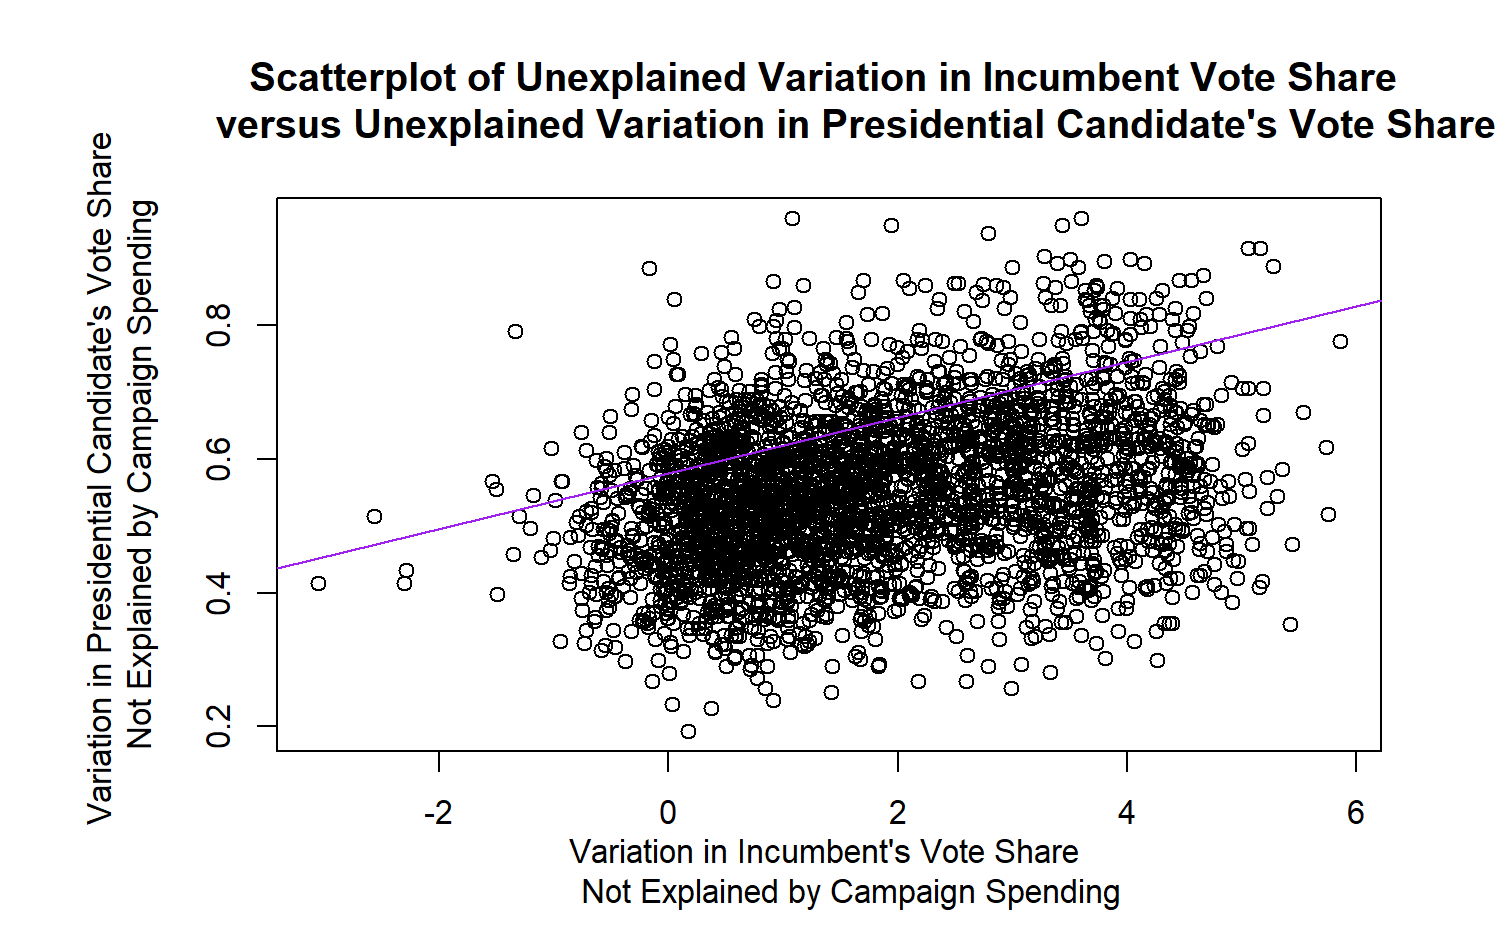
\includegraphics[width=1\textwidth]{Figure_4_1.png}
\end{figure} 
\newpage
\noindent\begin{enumerate}[left=0pt]
\setcounter{enumi}{2}			
\item Write the prediction equation.
\end{enumerate}
\vspace{0.25cm}
\noindent The fourth model is a bivariate model, meaning there is a single outcome and explanatory variable. \texttt{residuals.model.1} is the outcome variable, and \texttt{residuals.model.2} is the explanatory variable.

\begin{equation}
	\text{residuals.model.1} = \hat{\beta}_0 + \hat{\beta}_1 \cdot \text{residuals.model.2}
\end{equation}

\vspace{0.5cm} \noindent Inputting the values from the Model 4 Regression Output:
\begin{equation}
	\text{residuals.model.1} = 0 + 0.2569 \cdot \text{residuals.model.2}
\end{equation}

	
	\newpage	

\section*{Question 5}
\noindent What if the incumbent's vote share is affected by both the president's popularity and the difference in spending between incumbent and challenger? 
\noindent\begin{enumerate}[left=0pt]
\item Run a regression where the outcome variable is the incumbent's \texttt{voteshare} and the explanatory variables are \texttt{difflog} and \texttt{presvote}.
\end{enumerate}
\noindent Regression Model (5) for \texttt{voteshare}, \texttt{difflog}, and \texttt{presvote}: 
\noindent\lstinputlisting[language=R, firstline=151, lastline=152]{PS3_answers_DMcG.R}

\begin{table}[h!]
	\centering
	\caption{Summary of Regression Results for Model: voteshare ~ difflog + presvote}
	\vspace{0.25cm}
	\begin{tabular}{lccc}
		\toprule
		\textbf{Variable} & \textbf{Estimate} & \textbf{Std. Error} & \textbf{Significance} \\ 
		\midrule
		Intercept              & 0.4486 & 0.0063 & *** \\ 
		difflog                & 0.0355 & 0.0009 & *** \\ 
		presvote               & 0.2569 & 0.0118 & *** \\ 
		\midrule
		\textbf{Model Summary} & & & \\
		Residual Std. Error    & 0.07339  & (df = 3190) & \\ 
		Multiple R-squared     & 0.4496   & & \\ 
		Adjusted R-squared     & 0.4493   & & \\ 
		Number of Observations & 3193     & & \\ 
		\bottomrule
	\end{tabular}
\end{table}

\vspace{0.1cm}
\noindent\textbf{Significance Codes:} \\
*** $p < 0.001$, ** $p < 0.01$, * $p < 0.05$

\vspace{0.5cm} \begin{itemize}[left=0pt, label=\textbullet]
	\item The intercept of 0.4486 represents the average predicted vote share of the incumbent when both \texttt{difflog} and \texttt{presvote} are zero.
	\item There is a positive, statistically significant relationship between the log-transformed difference in campaign spending (\texttt{difflog}) and the incumbent’s vote share. Specifically, a one-unit increase in \texttt{difflog} is associated with an average increase of 3.55 percentage points in the incumbent’s vote share, holding \texttt{presvote} constant.
	\item There is also a positive, statistically significant relationship between the presidential candidate’s vote share (\texttt{presvote}) and the incumbent’s vote share. Specifically, a one-unit increase in \texttt{presvote} is associated with an average increase of 25.69 percentage points in the incumbent’s vote share, holding \texttt{difflog} constant.
	\item The multivariate regression model explains approximately 44.96\% of the variation in \texttt{voteshare}, as indicated by the Multiple R-squared of 0.4496, suggesting a moderate fit.
\end{itemize}


\noindent\begin{enumerate}[left=0pt]
\setcounter{enumi}{1}	
\item Write the prediction equation.
\end{enumerate}

\vspace{0.25cm}
\noindent The fourth model is a multivariate model, meaning there is a single outcome variable with multiple explanatory variables. \texttt{voteshare} is the outcome variable, while \texttt{difflog} and \texttt{presvote} are the explanatory variables.

\begin{equation}
	\text{voteshare} = \hat{\beta}_0 + \hat{\beta}_1 \cdot \text{difflog} + \hat{\beta}_2 \cdot \text{presvote}
\end{equation}

\vspace{0.5cm} \noindent Inputting the values from the Model 4 Regression Output:
\begin{equation}
	\text{voteshare} = 0.4486 + 0.0355 \cdot \text{difflog} + 0.2569 \cdot \text{presvote}
\end{equation}

\noindent\begin{enumerate}[left=0pt]
\setcounter{enumi}{1}	
\item What is it in this output that is identical to the output in Question 4? Why do you think this is the case?
\end{enumerate}
\begin{itemize}
	\item The coefficients for \texttt{residuals.model.2} in Model 4 and \texttt{presvote} in Model 5 are the same because they both measure the same underlying relationship.
	\item This relationship reflects the co-variation between the presidential candidate’s vote share (\texttt{presvote}) and the incumbent’s vote share (\texttt{voteshare}) that is not explained by the differences in campaign spending.
	\item In Model 4, this relationship is measured through the residuals (unexplained variation), while in Model 5, it captures the partial effect of \texttt{presvote} directly.
\end{itemize}




\end{document}
